\documentclass{plantilla}

\usepackage{multirow}
\usepackage{siunitx}
\usepackage{array}
% Ningun flotante puede quedar antes del lugar donde se lo declara: cada
% figura o tabla va despues del parrafo que la cita.
\usepackage{flafter}
\usepgfplotslibrary{fillbetween,groupplots}
\usetikzlibrary{calc}

% Mas espacio para flotantes en cada columna y menos paginas solo de figuras
\renewcommand{\topfraction}{0.85}
\renewcommand{\bottomfraction}{0.7}
\renewcommand{\textfraction}{0.1}
\renewcommand{\floatpagefraction}{0.85}
\renewcommand{\dbltopfraction}{0.9}
\renewcommand{\dblfloatpagefraction}{0.85}
\setcounter{topnumber}{3}
\setcounter{bottomnumber}{2}
\setcounter{totalnumber}{4}

\sisetup{
    output-decimal-marker = {,},
    group-digits = none,
    per-mode = symbol
}
\DeclareSIUnit{\ohm}{\ensuremath{\Omega}}

% Resultados de LTspice (generados por simulacion/correr_simulaciones.py)
% Generado por simulacion/correr_simulaciones.py
\newcommand{\simCTCon}{-0.0193373}
\newcommand{\simCTSin}{-0.0190457}
\newcommand{\simCTmVCon}{-0.959796}
\newcommand{\simCTmVSin}{-0.945807}
\newcommand{\simFactorRizo}{2.89641e-05}
\newcommand{\simIbPlena}{0.136576}
\newcommand{\simIbVeinticinco}{0.136576}
\newcommand{\simIrzVeinticinco}{20.6149}
\newcommand{\simIscCorto}{1.85124}
\newcommand{\simIzPlena}{20.4784}
\newcommand{\simIzVacio}{20.5509}
\newcommand{\simIzVeinticinco}{20.4784}
\newcommand{\simMejoraLinea}{72.7407}
\newcommand{\simPinVeinticinco}{13.1364}
\newcommand{\simPlVeinticinco}{2.48172}
\newcommand{\simPqCorto}{28.8207}
\newcommand{\simPqPlena}{7.75601}
\newcommand{\simPqUnAmper}{15.5198}
\newcommand{\simPqVeinticinco}{7.75601}
\newcommand{\simPregCorto}{17.4737}
\newcommand{\simPregPlena}{2.38466}
\newcommand{\simPregSinVeinticinco}{10.1579}
\newcommand{\simPregUnAmper}{4.63672}
\newcommand{\simPregVeinticinco}{2.38466}
\newcommand{\simRRPre}{38.7399}
\newcommand{\simRRReg}{75.0953}
\newcommand{\simRRSin}{76.4311}
\newcommand{\simRRTotal}{113.835}
\newcommand{\simRcar}{0.0213494}
\newcommand{\simRendimiento}{18.8919}
\newcommand{\simRendimientoSin}{19.6425}
\newcommand{\simRredCon}{0.00020566}
\newcommand{\simRredSin}{0.0149534}
\newcommand{\simRredSinDiez}{0.00706945}
\newcommand{\simRsal}{2.11933}
\newcommand{\simTjQNominal}{87.4668}
\newcommand{\simVbVeinticinco}{10.9818}
\newcommand{\simVbeAjMedio}{1.35267}
\newcommand{\simVbeErrMaxAj}{4.46921}
\newcommand{\simVbeErrMaxOrig}{789.691}
\newcommand{\simVbeHojaMedio}{1.354}
\newcommand{\simVbeOrigMedio}{0.771125}
\newcommand{\simVbeVeinticinco}{1.34505}
\newcommand{\simVceCorto}{15.565}
\newcommand{\simVceVeinticinco}{15.3632}
\newcommand{\simVefOut}{1.43762}
\newcommand{\simVefOutSin}{106.711}
\newcommand{\simViregCorto}{9.43501}
\newcommand{\simViregDiez}{8.53634}
\newcommand{\simViregMax}{9.66437}
\newcommand{\simViregMin}{9.60628}
\newcommand{\simViregPlena}{9.63679}
\newcommand{\simViregTolAlto}{10.177}
\newcommand{\simViregTolBajo}{9.09649}
\newcommand{\simViregTolDiezAlto}{8.53651}
\newcommand{\simViregTolDiezBajo}{8.49283}
\newcommand{\simViregTolDiezNom}{8.53634}
\newcommand{\simViregTolNom}{9.63679}
\newcommand{\simViregUnAmper}{9.55266}
\newcommand{\simViregVacio}{9.85978}
\newcommand{\simViregVeinticinco}{9.63679}
\newcommand{\simVoPlena}{4.96344}
\newcommand{\simVoSinVeinticinco}{4.96598}
\newcommand{\simVoUnAmper}{4.96273}
\newcommand{\simVoUnoCinco}{4.96203}
\newcommand{\simVoVacio}{4.9645}
\newcommand{\simVoVeinticinco}{4.96344}
\newcommand{\simVpVentana}{9.46348}
\newcommand{\simVrIn}{1.99999}
\newcommand{\simVrOut}{4.06694}
\newcommand{\simVrOutSin}{301.629}
\newcommand{\simVrVireg}{23.1225}
\newcommand{\simdViregCon}{58.0943}
\newcommand{\simdViregTemp}{13.4911}
\newcommand{\simdVoCarga}{1.05966}
\newcommand{\simdVoCompleta}{194.35}
\newcommand{\simdVoCon}{10.2078}
\newcommand{\simdVoSin}{742.524}
\newcommand{\simdVoSinCompleta}{2472.8}
\newcommand{\simdVoSinDiez}{350.88}
\newcommand{\simvalCargaAmplia}{2.2921}
\newcommand{\simvalCargaCentral}{0.715185}
\newcommand{\simvalDropout}{2.00053}
\newcommand{\simvalIq}{4.99521}
\newcommand{\simvalIscDiez}{1.8238}
\newcommand{\simvalIscTreintaycinco}{0.297642}
\newcommand{\simvalIscVeinticinco}{0.936742}
\newcommand{\simvalLineaAmplia}{3.01653}
\newcommand{\simvalLineaCentral}{0.701998}
\newcommand{\simvalRR}{75.1048}
\newcommand{\simvalTempco}{-1.22348}
\newcommand{\simvalVo}{4.9635}

% \val{decimales}{\simXxx}: numero simulado redondeado
\newcommand{\val}[2]{\num[round-mode=places,round-precision=#1]{#2}}
% \valu{decimales}{\simXxx}{unidad}: numero simulado con unidad
\newcommand{\valu}[3]{\SI[round-mode=places,round-precision=#1]{#2}{#3}}
\newcommand{\Vireg}{V_{i,\mathrm{reg}}}
\newcommand{\Vp}{V_{P}}

\materia{Electrónica Aplicada II}
\comision{4R2}
\titulo{Actividad Evaluativa Unidad 6: Fuente de \SI{5}{\volt} con LM7805 y Etapa Prereguladora (Consigna 6)}
\autores{Grupo 6: Ernst Pedro (400624), López Demichelis Alejo (401900),\\ Polizze Tomás (400793), Rao Valentino (402308)}

\begin{document}

\maketitle

\begin{abstract}
Se diseña una fuente de \SI{5}{\volt} y \SI{0,5}{\ampere} con el regulador integrado LM7805 a partir de una fuente primaria de \SI{25}{\volt} de continua. Para que el regulador trabaje con una entrada de \SI{8}{\volt} a \SI{12}{\volt}, donde su regulación de línea es mejor, se antepone una etapa prereguladora serie formada por un Darlington TIP122 y un Zener 1N4741A de \SI{11}{\volt}, según la Fig.~6-71 del apunte de la cátedra. Se selecciona el transistor con su ganancia mínima garantizada, se verifica su punto de trabajo en el área de operación segura y se calculan los disipadores del transistor y del regulador. Todo el diseño se simula en LTspice, con los modelos que publican los fabricantes del transistor (con la $V_{BE}$ ajustada a su hoja de datos) y del diodo de protección, un modelo a nivel transistor del LM7805 validado contra su hoja de datos y un modelo del Zener ajustado a la suya. Con la entrada del regulador en \valu{2}{\simViregVeinticinco}{\volt}, una variación de $\pm\SI{10}{\percent}$ de la fuente primaria cambia la salida en \valu{1}{\simdVoCon}{\micro\volt}, contra \valu{0}{\simdVoSin}{\micro\volt} cuando el LM7805 se conecta directo a \SI{25}{\volt}. Se informan todos los parámetros de calidad definidos en el apunte.
\end{abstract}

\begin{IEEEkeywords}
Fuente lineal, LM7805, etapa prereguladora, regulación de línea, área de operación segura, disipador, LTspice.
\end{IEEEkeywords}

\section{Introducción}

\subsection{Consigna e interpretación}
La Consigna 6 de la actividad evaluativa de la Unidad 6 pide:
\begin{quote}
\emph{``Diseñar y calcular una fuente de alimentación con un regulador lineal integrado LM7805. Se dispone de una fuente primaria de \SI{25}{\volt} dc. A los fines de mejorar la regulación del voltaje de línea es necesario un rango de $V_{in} = \SI{8}{}$--$\SI{12}{\volt}$. Incluir en el diseño una etapa que cumpla con este objetivo. Verificar mediante simulación la regulación de línea para $V_{in} = \SI{25}{\volt}$ y $V_{in} = \SI{10}{\volt}$. Seleccionar transistor, verificar punto de operación según SOA e incluir eventual cálculo de disipador. Obtener todos los parámetros de calidad de fuentes de alimentación.''}
\end{quote}

En el enunciado, $V_{in}$ es la tensión de entrada del regulador: el rango de \SI{8}{\volt} a \SI{12}{\volt} es el que la hoja de datos del LM7805 usa para especificar su mejor regulación de línea. Por eso la verificación pedida se interpreta como la comparación entre dos situaciones: el LM7805 conectado directo a la fuente primaria ($V_{in} = \SI{25}{\volt}$) y el LM7805 alimentado a través de la etapa prereguladora, que lleva su entrada a unos \SI{10}{\volt}. Para cubrir también la otra lectura posible, se simula el caso en que la propia fuente primaria baja a \SI{10}{\volt} (Sección~\ref{sec:linea}).

\subsection{Especificaciones de diseño}
La consigna no fija la corriente de carga. Se adopta $I_{L,\max} = \SI{0,5}{\ampere}$, que es la corriente con la que la hoja de datos especifica las características eléctricas del regulador~\cite{ua78}, y $I_{L,\min} = 0$, como establece el apunte para la regulación de carga~\cite[Sec.~6-6-3b]{ap2}. La Tabla~\ref{tab:especificaciones} resume el resto de los datos de partida. La variación de $\pm\SI{10}{\percent}$ de la fuente primaria es la que el apunte toma para la regulación de red~\cite[Sec.~6-6-3a]{ap2}, y la temperatura ambiente máxima y la de juntura de diseño son las del Ejemplo~9 del apunte~\cite[Sec.~6-8-3b]{ap2}. El rizado de prueba de \SI{2}{\volt} pico a pico a \SI{100}{\hertz} representa una fuente primaria obtenida con un rectificador de onda completa de \SI{50}{\hertz}; se usa solo para medir el rechazo de rizado.

\begin{table}[!htb]
\centering
\caption{Especificaciones adoptadas para el diseño.}
\label{tab:especificaciones}
\begin{tabular}{lc}
\toprule
\textbf{Parámetro} & \textbf{Valor} \\
\midrule
Fuente primaria $\Vp$ & \SI{25}{\volt} $\pm\SI{10}{\percent}$ (\SI{22,5}{} a \SI{27,5}{\volt}) \\
Tensión de salida $V_O$ & \SI{5}{\volt} (LM7805) \\
Corriente de carga $I_L$ & \SI{0}{} a \SI{0,5}{\ampere} \\
Entrada del regulador $\Vireg$ & \SI{8}{} a \SI{12}{\volt} \\
Temperatura ambiente máxima $T_a$ & \SI{40}{\celsius} \\
Temperatura de juntura de diseño $T_J$ & \SI{100}{\celsius} \\
Rizado de prueba en $\Vp$ & \SI{2}{\volt} pico a pico, \SI{100}{\hertz} \\
\bottomrule
\end{tabular}
\end{table}

\subsection{El regulador LM7805}
Los reguladores de la familia 78XX integran en un mismo chip el elemento serie (un par Darlington), una referencia de tensión, la red de muestreo, el amplificador de error y tres protecciones: limitación de corriente, protección de área segura, que reduce la corriente disponible cuando crece la diferencia $V_I - V_O$, y corte por temperatura~\cite[Sec.~6-9-1 y 6-9-2]{ap3}, \cite[Sec.~15-8.3]{coughlin}. La Fig.~\ref{fig:bloques_7805} muestra el diagrama en bloques y la Tabla~\ref{tab:datasheet_7805} los datos de la hoja de datos que se usan en este trabajo.

\begin{figure}[!htb]
\centering
\resizebox{\columnwidth}{!}{%
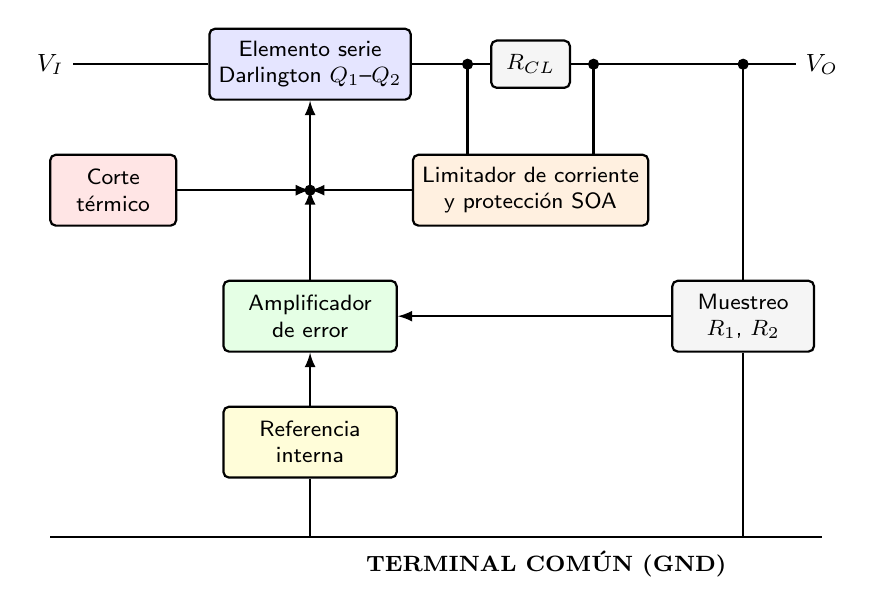
\begin{tikzpicture}[
    block/.style={draw, thick, rectangle, rounded corners=2pt, minimum height=0.9cm, align=center, font=\footnotesize\sffamily, fill=gray!8},
    line/.style={thick, -latex}
]
    % camino de potencia
    \node[font=\small] (vin) at (-0.9, 3.4) {$V_I$};
    \node[font=\small] (vout) at (8.9, 3.4) {$V_O$};
    \node[block, fill=blue!10, minimum width=2.4cm] (pass) at (2.4, 3.4) {Elemento serie\\Darlington $Q_1$--$Q_2$};
    \node[block, minimum width=1.0cm, minimum height=0.6cm] (rcl) at (5.2, 3.4) {$R_{CL}$};
    \draw[thick] (vin) -- (pass.west);
    \draw[thick] (pass.east) -- (rcl.west);
    \draw[thick] (rcl.east) -- (vout);
    % nodo de excitacion de base
    \coordinate (J) at (2.4, 1.8);
    \draw[line] (J) -- (pass.south);
    \filldraw (J) circle (1.8pt);
    % protecciones
    \node[block, fill=red!10, minimum width=1.6cm] (term) at (-0.1, 1.8) {Corte\\térmico};
    \draw[line] (term.east) -- (J);
    \node[block, fill=orange!12, minimum width=2.9cm] (lim) at (5.2, 1.8) {Limitador de corriente\\y protección SOA};
    \draw[line] (lim.west) -- (J);
    \filldraw (4.4, 3.4) circle (1.8pt);
    \filldraw (6.0, 3.4) circle (1.8pt);
    \draw[thick] (4.4, 3.4) -- (4.4, 2.25);
    \draw[thick] (6.0, 3.4) -- (6.0, 2.25);
    % lazo de regulacion
    \node[block, fill=green!10, minimum width=2.2cm] (amp) at (2.4, 0.2) {Amplificador\\de error};
    \draw[line] (amp.north) -- (J);
    \node[block, fill=yellow!15, minimum width=2.2cm] (ref) at (2.4, -1.4) {Referencia\\interna};
    \draw[line] (ref.north) -- (amp.south);
    \node[block, minimum width=1.8cm] (samp) at (7.9, 0.2) {Muestreo\\$R_1$, $R_2$};
    \filldraw (7.9, 3.4) circle (1.8pt);
    \draw[thick] (7.9, 3.4) -- (samp.north);
    \draw[line] (samp.west) -- (amp.east);
    % masa
    \draw[thick] (-0.9, -2.6) -- (8.9, -2.6);
    \draw[thick] (ref.south) -- (2.4, -2.6);
    \draw[thick] (samp.south) -- (7.9, -2.6);
    \node[font=\footnotesize\bfseries] at (5.4, -2.95) {TERMINAL COMÚN (GND)};
\end{tikzpicture}%
}
\caption{Diagrama en bloques del regulador LM7805 (adaptado de \cite[Fig.~6-55 a 6-57]{ap3}).}
\label{fig:bloques_7805}
\end{figure}

\begin{table}[!htb]
\centering
\caption{Características del $\mu$A7805C a $T_J = \SI{25}{\celsius}$, $V_I = \SI{10}{\volt}$ e $I_O = \SI{500}{\milli\ampere}$, salvo indicación~\cite{ua78}.}
\label{tab:datasheet_7805}
\footnotesize
\setlength{\tabcolsep}{3.5pt}
\begin{tabular}{@{}>{\raggedright}p{3.9cm}ccc@{}}
\toprule
\textbf{Parámetro y condición} & \textbf{Mín.} & \textbf{Típ.} & \textbf{Máx.} \\
\midrule
Tensión de salida, $I_O = \SI{5}{\milli\ampere}$ a \SI{1}{\ampere}, $V_I = \SI{7}{}$ a \SI{20}{\volt} & \SI{4,8}{\volt} & \SI{5}{\volt} & \SI{5,2}{\volt} \\
Regulación de línea, $V_I = \SI{7}{}$ a \SI{25}{\volt} & -- & \SI{3}{\milli\volt} & \SI{100}{\milli\volt} \\
Regulación de línea, $V_I = \SI{8}{}$ a \SI{12}{\volt} & -- & \SI{1}{\milli\volt} & \SI{50}{\milli\volt} \\
Rechazo de rizado, $V_I = \SI{8}{}$ a \SI{12}{\volt}, \SI{120}{\hertz} & \SI{62}{\deci\bel} & \SI{78}{\deci\bel} & -- \\
Regulación de carga, $I_O = \SI{5}{\milli\ampere}$ a \SI{1,5}{\ampere} & -- & \SI{15}{\milli\volt} & \SI{100}{\milli\volt} \\
Regulación de carga, $I_O = \SI{250}{}$ a \SI{750}{\milli\ampere} & -- & \SI{5}{\milli\volt} & \SI{50}{\milli\volt} \\
Resistencia de salida, $f = \SI{1}{\kilo\hertz}$ & -- & \SI{0,017}{\ohm} & -- \\
Coef.\ de temperatura, $I_O = \SI{5}{\milli\ampere}$ & -- & \SI{-1,1}{\milli\volt\per\celsius} & -- \\
Tensión de \emph{dropout}, $I_O = \SI{1}{\ampere}$ & -- & \SI{2}{\volt} & -- \\
Corriente de polarización & -- & \SI{4,2}{\milli\ampere} & \SI{8}{\milli\ampere} \\
Corriente de cortocircuito & -- & \SI{750}{\milli\ampere} & -- \\
Corriente de pico & -- & \SI{2,2}{\ampere} & -- \\
Tensión de entrada recomendada & \SI{7}{\volt} & -- & \SI{25}{\volt} \\
$R_{\theta JP}$, TO-220, juntura a aleta & -- & \SI{3}{\celsius\per\watt} & -- \\
\bottomrule
\end{tabular}
\end{table}

\subsection{Por qué conviene una entrada de \SI{8}{} a \SI{12}{\volt}}
La hoja de datos da dos valores de regulación de línea. Para $V_I$ entre \SI{7}{} y \SI{25}{\volt} la salida cambia \SI{3}{\milli\volt} típicos, y si la entrada se limita a la zona central, de \SI{8}{} a \SI{12}{\volt}, el cambio baja a \SI{1}{\milli\volt}~\cite[Sec.~6-9-3]{ap3}. Además:
\begin{itemize}
    \item El límite inferior surge del margen que necesita el regulador para que su elemento serie no salga de la zona activa: $V_{I,\min} = V_O + \text{margen} = \SI{5}{\volt} + \SI{3}{\volt} = \SI{8}{\volt}$~\cite[Ec.~15-8 y Sec.~15-9.2]{coughlin}. Con \SI{8}{\volt} queda \SI{1}{\volt} por encima del \emph{dropout} de \SI{2}{\volt}.
    \item Conectado directo a \SI{25}{\volt}, el LM7805 trabaja en el límite de su tensión de entrada recomendada y debe disipar $(25 - 5)\,\si{\volt} \times \SI{0,5}{\ampere} = \SI{10}{\watt}$. Con la entrada en unos \SI{10}{\volt}, la disipación baja a unos \SI{2,5}{\watt} y el resto de la caída la toma un transistor externo, más fácil de refrigerar.
\end{itemize}

\section{Diseño de la etapa prereguladora}

\subsection{Topología}
El apunte presenta dos circuitos para alimentar un regulador integrado desde una tensión mayor que la que admite, ambos con un transistor serie y un diodo Zener~\cite[Sec.~6-9-5g]{ap3}:
\begin{enumerate}
    \item \textbf{Zener entre base y masa (Fig.~6-71).} El Zener fija la tensión de base y el transistor trabaja como seguidor de emisor:
    \begin{equation}
        \Vireg = V_Z - V_{BE}.
        \label{eq:vireg}
    \end{equation}
    El exceso de tensión $\Vp - \Vireg$ cae entre colector y emisor, y las variaciones de $\Vp$ llegan a la base atenuadas por el divisor que forman $R_Z$ y la impedancia dinámica del Zener.
    \item \textbf{Zener entre colector y base (Fig.~6-72).} Resta a la entrada una tensión fija: $\Vireg = \Vp - (V_Z + V_{BE})$. Toda variación de $\Vp$ pasa sin atenuar a la entrada del regulador, y si $\Vp$ baja de $V_Z + V_{BE}$ el circuito deja de conducir.
\end{enumerate}
Como el objetivo es mejorar la regulación de línea, se adopta el circuito de la Fig.~6-71. La Fig.~\ref{fig:esquematico} muestra el circuito completo.

\begin{figure*}[t]
\centering
\begin{circuitikz}[scale=0.92, transform shape, >=latex]
    % Fuente primaria
    \draw (0,0) node[ground]{} to[V, v<={$\Vp = \SI{25}{\volt}$}] (0,4)
          to[short, -*] (2,4) coordinate (vp);
    % Rz y Zener
    \draw (vp) to[R, l^={$R_Z$\\\SI{680}{\ohm}\\\SI{1}{\watt}}, align=left] (2,2) coordinate (b);
    \draw (2,0) node[ground]{} to[zzDo, l_={$D_Z$\\1N4741A\\\SI{11}{\volt}}, align=left, -*] (b);
    % Transistor de paso
    \draw (vp) -- (3.6,4);
    \node[npn, rotate=90] (Q1) at (4.4,4) {};
    \node[above, font=\small] at (4.4,4.6) {$Q_1$: TIP122};
    \draw (3.6,4) -- (Q1.C);
    \draw (b) -| (Q1.B);
    \node[right, font=\footnotesize] at (4.4,2.6) {$I_B$};
    % Nodo Vi,reg
    \draw (Q1.E) to[short, -*] (7,4) coordinate (vi);
    \node[above, font=\small] at (7,4.05) {$\Vireg$};
    \draw (vi) to[C] (7,0) node[ground]{};
    \node[left, align=right, font=\small] at (6.55,2) {$C_1$\\\SI{0,33}{\micro\farad}};
    % Regulador
    \draw (vi) -- (8.6,4);
    \draw[thick, fill=blue!6] (8.6,3.3) rectangle (11,4.7);
    \node[font=\bfseries\small] at (9.8,4.15) {LM7805};
    \node[font=\scriptsize] at (9.0,3.75) {IN};
    \node[font=\scriptsize] at (10.6,3.75) {OUT};
    \node[font=\scriptsize] at (9.8,3.5) {GND};
    \draw (9.8,3.3) -- (9.8,0) node[ground]{};
    % Diodo de proteccion
    \draw (11.6,4) -- (11.6,5.5) to[D, l_={$D_1$: 1N4002}] (8,5.5) -- (8,4);
    \filldraw (8,4) circle (1.8pt);
    % Salida
    \draw (11,4) to[short, -*] (11.6,4) to[short, -*] (13,4) coordinate (c2);
    \draw (c2) to[C] (13,0) node[ground]{};
    \node[left, align=right, font=\small] at (12.55,2) {$C_2$\\\SI{0,1}{\micro\farad}};
    \draw (c2) to[short, -*] (15,4) coordinate (vo);
    \draw (vo) to[R, l_={Carga\\\SI{0}{}--\SI{0,5}{\ampere}}, align=right, v^>=$V_O$] (15,0) node[ground]{};
    \draw (vo) to[short, -o] (16.2,4) node[right] {\SI{5}{\volt}};
    % Recuadro de la etapa
    \draw[dashed, rounded corners=4pt, color=orange!80!black, thick] (1.0,0.25) rectangle (5.6,5.25);
    \node[font=\footnotesize\bfseries, color=orange!80!black] at (3.3,5.5) {Etapa prereguladora};
\end{circuitikz}
\caption{Fuente de \SI{5}{\volt} con etapa prereguladora serie. Es el mismo circuito que el de los esquemáticos de LTspice (\texttt{simulacion/c6\_*.asc}).}
\label{fig:esquematico}
\end{figure*}

\subsection{Tensión de entrada del regulador}
Se busca que $\Vireg$ quede en el centro de la ventana de \SI{8}{} a \SI{12}{\volt}, en torno a \SI{10}{\volt}, que además es la tensión de ensayo de la hoja de datos. Así queda margen para la tolerancia del Zener, para la dispersión de $V_{BE}$ y para el rizado. Con $\Vireg = \SI{10}{\volt}$, el regulador trabaja con $\Vireg - V_O = \SI{5}{\volt}$, por encima de los \SI{3}{\volt} de margen mínimo~\cite[Ec.~15-8]{coughlin}. En el ejemplo de diseño del apunte se adopta un criterio parecido: \SI{4}{\volt} sobre el regulador y $\Vireg = \SI{9}{\volt}$~\cite[Sec.~6-9-5h]{ap3}.

\subsection{Selección del transistor de paso}
\label{sec:seleccion_transistor}
Por el transistor circula la corriente de carga más la de polarización del regulador:
\begin{equation}
    I_{C,\max} = I_{L,\max} + I_{d,\max} = \SI{0,5}{\ampere} + \SI{8}{\milli\ampere} = \SI{0,508}{\ampere}.
\end{equation}
La tensión y la potencia que debe soportar se calculan en la Sección~\ref{sec:soa}. Lo que define la elección es la corriente de base, porque el Zener debe absorberla sin salir de su zona de trabajo. El apunte fija la corriente del Zener en diez veces la corriente de base máxima~\cite[Sec.~6-9-5h]{ap3}:
\begin{equation}
    I_{Z} \geq 10\, I_{B,\max} = 10\, \frac{I_{C,\max}}{h_{FE,\min}}.
    \label{eq:criterio_iz}
\end{equation}
En el ejemplo del apunte se usa un TIP31A con la ganancia típica de su curva, $h_{FE} = 100$. Pero la ganancia garantizada del TIP31C es mucho menor: $h_{FE} \geq 25$ con $I_C = \SI{1}{\ampere}$ y $V_{CE} = \SI{4}{\volt}$~\cite{tip31}. En el peor caso, $I_{B,\max} = \SI{0,508}{\ampere}/25 = \SI{20,3}{\milli\ampere}$ y la Ec.~\eqref{eq:criterio_iz} pide $I_Z \geq \SI{203}{\milli\ampere}$. Con la fuente primaria en su mínimo de \SI{22,5}{\volt} eso da $R_Z = (22{,}5 - 11)\,\si{\volt}/\SI{223}{\milli\ampere} \approx \SI{52}{\ohm}$, y sin carga y con la primaria en \SI{27,5}{\volt} el Zener disiparía unos \SI{3,5}{\watt} y $R_Z$ más de \SI{5}{\watt}. Un transistor simple no sirve.

Se elige el Darlington \textbf{TIP122}, que garantiza $h_{FE} \geq 1000$ con $I_C = \SI{0,5}{\ampere}$ y $V_{CE} = \SI{3}{\volt}$~\cite{tip120}. Su corriente de base máxima es
\begin{equation}
    I_{B,\max} = \frac{\SI{0,508}{\ampere}}{1000} = \SI{0,51}{\milli\ampere},
\end{equation}
y alcanza con $I_Z \geq \SI{5,1}{\milli\ampere}$. La Tabla~\ref{tab:transistores} compara ambos transistores. La contrapartida del Darlington es que su $V_{BE}$ es la suma de dos junturas, de unos \SI{1,4}{\volt}, lo que se tiene en cuenta al elegir el Zener.

\begin{table}[!htb]
\centering
\caption{Comparación de los transistores considerados~\cite{tip31,tip120}.}
\label{tab:transistores}
\resizebox{\columnwidth}{!}{%
\begin{tabular}{lccc}
\toprule
\textbf{Parámetro} & \textbf{Requerido} & \textbf{TIP31C} & \textbf{TIP122} \\
\midrule
$V_{CEO}$ & $> \SI{27,5}{\volt}$ & \SI{100}{\volt} & \SI{100}{\volt} \\
$I_C$ continua & \SI{0,508}{\ampere} & \SI{3}{\ampere} & \SI{5}{\ampere} \\
$P_D$ ($T_C = \SI{25}{\celsius}$) & \SI{9,5}{\watt} & \SI{40}{\watt} & \SI{65}{\watt} \\
$h_{FE}$ mínima & -- & 25 (\SI{1}{\ampere}) & 1000 (\SI{0,5}{\ampere}) \\
$I_{B,\max}$ a \SI{0,508}{\ampere} & -- & \SI{20,3}{\milli\ampere} & \SI{0,51}{\milli\ampere} \\
$R_{\theta JC}$ & -- & \SI{3,125}{\celsius\per\watt} & \SI{1,92}{\celsius\per\watt} \\
$R_{\theta JA}$ & -- & \SI{62,5}{\celsius\per\watt} & \SI{62,5}{\celsius\per\watt} \\
\bottomrule
\end{tabular}%
}
\end{table}

\subsection{Selección del diodo Zener}
De la Ec.~\eqref{eq:vireg}, con $V_{BE} \approx \SI{1,4}{\volt}$:
\begin{equation}
    V_Z = \Vireg + V_{BE} \approx \SI{10}{\volt} + \SI{1,4}{\volt} = \SI{11,4}{\volt}.
\end{equation}
Se elige el \textbf{1N4741A}: $V_Z = \SI{11}{\volt} \pm \SI{5}{\percent}$ con $I_{ZT} = \SI{23}{\milli\ampere}$, $Z_{ZT} \leq \SI{8}{\ohm}$, $Z_{ZK} \leq \SI{700}{\ohm}$ con $I_{ZK} = \SI{0,25}{\milli\ampere}$ y \SI{1}{\watt} de potencia~\cite{zener}. Con el valor nominal resulta $\Vireg \approx \SI{9,6}{\volt}$. En el peor caso, con $V_Z$ entre \SI{10,45}{} y \SI{11,55}{\volt} y $V_{BE}$ entre \SI{1,2}{} y \SI{1,6}{\volt}, $\Vireg$ queda entre \SI{8,85}{} y \SI{10,35}{\volt}, siempre dentro de la ventana. El Zener de \SI{10}{\volt} (1N4740A) dejaría $\Vireg$ en unos \SI{8,6}{\volt}, demasiado cerca del límite inferior.

\subsection{Cálculo de $R_Z$}
Para que el Zener trabaje con baja impedancia dinámica se fija su corriente cerca de $I_{ZT}$, en unos \SI{20}{\milli\ampere} con la primaria en \SI{25}{\volt} y plena carga:
\begin{equation}
    R_Z = \frac{\Vp - V_Z}{I_Z + I_{B,\max}} = \frac{\SI{25}{\volt} - \SI{11}{\volt}}{\SI{20}{\milli\ampere} + \SI{0,51}{\milli\ampere}} = \SI{683}{\ohm}.
\end{equation}
Se adopta $R_Z = \SI{680}{\ohm}$. El valor no supera el máximo que da la Ec.~6-49 del apunte~\cite{ap2}, en la que la corriente de base cumple el papel de la corriente de carga del Zener y $I_{Z,\min} = 10\,I_{B,\max}$:
\begin{equation}
    R_{Z,\max} = \frac{V_{P,\min} - V_Z}{I_{Z,\min} + I_{B,\max}} = \frac{\SI{22,5}{\volt} - \SI{11}{\volt}}{\SI{5,1}{\milli\ampere} + \SI{0,51}{\milli\ampere}} = \SI{2,05}{\kilo\ohm}.
\end{equation}
Con la primaria al mínimo y plena carga, el Zener conduce $(22{,}5 - 11)/680 - 0{,}51 = \SI{16,4}{\milli\ampere}$. La corriente máxima se da con la primaria en \SI{27,5}{\volt} y sin carga, cuando $I_B \approx 0$ (Ec.~6-51), y de ella sale la potencia máxima del Zener (Ec.~6-50):
\begin{align}
    I_{Z,\max} &= \frac{\SI{27,5}{\volt} - \SI{11}{\volt}}{\SI{680}{\ohm}} = \SI{24,3}{\milli\ampere}, \\
    P_{Z,\max} &= I_{Z,\max}\, V_Z = \SI{0,27}{\watt}.
\end{align}
El 1N4741A admite \SI{1}{\watt}, casi cuatro veces más, y cumple el factor de seguridad de 2 que aconseja la Ec.~6-55~\cite{ap2}. En $R_Z$ se disipan, como máximo, $(27{,}5 - 11)^2/680 = \SI{0,40}{\watt}$, por lo que se usa una resistencia de \SI{1}{\watt}.

La etapa también atenúa el rizado de la fuente primaria. Según la Ec.~6-76 del apunte~\cite{ap2}, el rizado que llega a la base es
\begin{equation}
    V_{Z,pp} = V_{r,pp} \frac{Z_{ZT}}{R_Z + Z_{ZT}} = \SI{2}{\volt} \times \frac{\SI{7}{\ohm}}{\SI{687}{\ohm}} = \SI{20,4}{\milli\volt},
    \label{eq:rizado_zener}
\end{equation}
una atenuación de \SI{39,8}{\deci\bel} antes del regulador.

\subsection{Capacitores y diodo de protección}
$C_1 = \SI{0,33}{\micro\farad}$ y $C_2 = \SI{0,1}{\micro\farad}$, cerámicos, van soldados junto a los terminales del regulador. Son los del circuito básico del apunte~\cite[Fig.~6-62]{ap3} y los mismos con que la hoja de datos mide todas sus características~\cite{ua78}: $C_1$ filtra transitorios en la entrada y $C_2$ evita oscilaciones y mejora la respuesta transitoria. El diodo $D_1$ (1N4002), entre salida y entrada, protege al regulador si su entrada queda en cortocircuito o cae antes que la salida, siguiendo la fuente de \SI{5}{\volt} del Coughlin~\cite[Fig.~15-11]{coughlin}. La Tabla~\ref{tab:componentes} lista los componentes.

\begin{table}[!htb]
\centering
\caption{Lista de componentes.}
\label{tab:componentes}
\footnotesize
\begin{tabular}{@{}l>{\raggedright}p{3.3cm}>{\raggedright\arraybackslash}p{3.4cm}@{}}
\toprule
\textbf{Ref.} & \textbf{Componente} & \textbf{Observaciones} \\
\midrule
$Q_1$ & TIP122 (Darlington NPN) & Disipador Aluel ZD-28 de \SI{75}{\milli\meter}, con mica y grasa \\
$U_1$ & LM7805 ($\mu$A7805C), TO-220 & Disipador Aluel 2125D \\
$D_Z$ & 1N4741A, \SI{11}{\volt}, \SI{1}{\watt} & -- \\
$R_Z$ & \SI{680}{\ohm}, \SI{5}{\percent} & \SI{1}{\watt} \\
$C_1$ & \SI{0,33}{\micro\farad}, cerámico, \SI{50}{\volt} & Junto a IN y GND de $U_1$ \\
$C_2$ & \SI{0,1}{\micro\farad}, cerámico, \SI{50}{\volt} & Junto a OUT y GND de $U_1$ \\
$D_1$ & 1N4002 & Protección de $U_1$ \\
\bottomrule
\end{tabular}
\end{table}

\section{Punto de trabajo, SOA y disipadores}
\label{sec:soa}

\subsection{Exigencias sobre el transistor}
Siguiendo el apunte~\cite[Sec.~6-8-3]{ap2}, el transistor se verifica con su tensión, corriente y potencia máximas. En funcionamiento normal, la mayor tensión colector-emisor se da con la fuente primaria al máximo y $\Vireg$ al mínimo (Ec.~6-77):
\begin{equation}
    V_{CE,\max} = V_{P,\max} - V_{i,\mathrm{reg},\min} = \SI{27,5}{\volt} - \SI{8,85}{\volt} = \SI{18,65}{\volt},
\end{equation}
y la potencia máxima en el colector es (Ec.~6-63)
\begin{equation}
    P_{C,\max} = V_{CE,\max}\, I_{C,\max} = \SI{18,65}{\volt} \times \SI{0,508}{\ampere} = \SI{9,5}{\watt}.
\end{equation}
Al encender la fuente, mientras se cargan $C_1$ y $C_2$, el transistor puede llegar a ver toda la tensión de la primaria, \SI{27,5}{\volt}. El TIP122 soporta \SI{100}{\volt}, \SI{5}{\ampere} y \SI{65}{\watt}~\cite{tip120}, con amplio margen en las tres magnitudes.

En la condición nominal ($\Vp = \SI{25}{\volt}$, $I_L = \SI{0,5}{\ampere}$), la simulación da $V_{CE} = \valu{2}{\simVceVeinticinco}{\volt}$ y $P_C = \valu{2}{\simPqVeinticinco}{\watt}$ (Sección~\ref{sec:sim}).

\subsection{Área de operación segura}
La Fig.~\ref{fig:soa} reproduce la curva de continua del área de operación segura del TIP122, digitalizada de la Fig.~6 de su hoja de datos~\cite{tip120}. Tiene los tramos que describe el apunte~\cite[Sec.~6-8-3c]{ap2}: límite de corriente por los hilos de conexión (\SI{5}{\ampere}), límite térmico de \SI{65}{\watt} a $T_C = \SI{25}{\celsius}$, límite de segunda ruptura desde unos \SI{20}{\volt} y límite de tensión en $V_{CEO} = \SI{100}{\volt}$. Como la curva vale para $T_C = \SI{25}{\celsius}$, se agrega la curva reducida para la temperatura de carcasa con el disipador elegido más adelante, $T_C \approx \SI{80}{\celsius}$, en la que la potencia admisible baja a $65 - 0{,}52\times(80 - 25) \approx \SI{36}{\watt}$.

Los puntos de trabajo nominal ($Q_{\mathrm{nom}}$) y de peor caso ($Q_{\max}$) quedan muy por debajo de ambas curvas, lejos de la zona de segunda ruptura. El punto de cortocircuito en la salida ($Q_{cc}$, \valu{2}{\simIscCorto}{\ampere} según la simulación) también queda dentro del área segura, aunque no puede sostenerse en el tiempo con el disipador elegido (Sección~\ref{sec:corto}).

\begin{figure}[!htb]
\centering
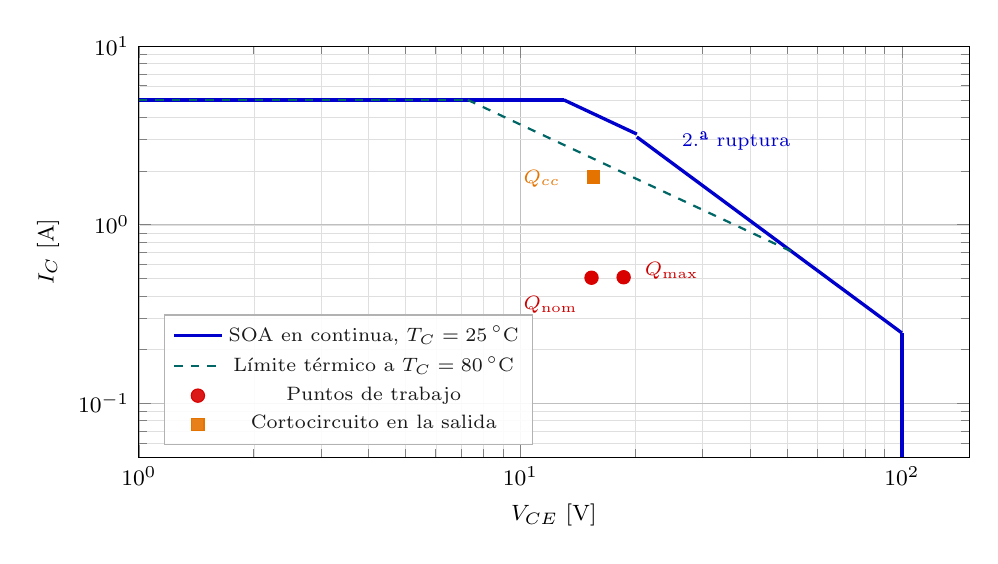
\begin{tikzpicture}
\begin{loglogaxis}[
    width=\columnwidth, height=6.8cm,
    xlabel={$V_{CE}$ [\si{\volt}]}, ylabel={$I_C$ [\si{\ampere}]},
    xmin=1, xmax=150, ymin=0.05, ymax=10,
    grid=both, grid style={line width=.1pt, draw=gray!25},
    major grid style={line width=.2pt, draw=gray!50},
    legend pos=south west,
    legend style={font=\scriptsize, fill=white, fill opacity=0.9, draw=gray!60},
    tick label style={font=\footnotesize}, label style={font=\footnotesize},
]
    \addplot[blue!80!black, very thick] coordinates {(1,5) (13,5)};
    \addlegendentry{SOA en continua, $T_C = \SI{25}{\celsius}$}
    \addplot[blue!80!black, very thick, domain=13:20.2, samples=20, forget plot] {65/x};
    \addplot[blue!80!black, very thick, domain=20.2:100, samples=40, forget plot] {3.1*(20.2/x)^1.58};
    \addplot[blue!80!black, very thick, forget plot] coordinates {(100,0.247) (100,0.05)};
    \addplot[teal!80!black, thick, dashed, domain=7.28:51.6, samples=40] {36.4/x};
    \addlegendentry{Límite térmico a $T_C = \SI{80}{\celsius}$}
    \addplot[teal!80!black, thick, dashed, forget plot] coordinates {(1,5) (7.28,5)};
    \addplot[only marks, mark=*, mark size=2.4pt, red!85!black] coordinates {(\simVceVeinticinco, 0.505) (18.65, 0.508)};
    \addlegendentry{Puntos de trabajo}
    \addplot[only marks, mark=square*, mark size=2.2pt, orange!90!black] coordinates {(\simVceCorto, \simIscCorto)};
    \addlegendentry{Cortocircuito en la salida}
    \node[anchor=north, font=\scriptsize, text=red!80!black] at (axis cs:12,0.45) {$Q_{\mathrm{nom}}$};
    \node[anchor=west, font=\scriptsize, text=red!80!black] at (axis cs:20,0.55) {$Q_{\max}$};
    \node[anchor=east, font=\scriptsize, text=orange!90!black] at (axis cs:13.5,1.82) {$Q_{cc}$};
    \node[anchor=south west, font=\scriptsize, text=blue!80!black] at (axis cs:25,2.3) {2.ª ruptura};
\end{loglogaxis}
\end{tikzpicture}
\caption{Área de operación segura en continua del TIP122 (digitalizada de~\cite[Fig.~6]{tip120}) y puntos de trabajo del diseño.}
\label{fig:soa}
\end{figure}

\subsection{Disipador del transistor}
La transferencia de calor se modela con el circuito térmico de la Fig.~\ref{fig:circuito_termico}, en el que las resistencias térmicas quedan en serie (Ec.~6-79 a 6-81 del apunte~\cite{ap2}):
\begin{equation}
    \frac{T_J - T_a}{P_C} = R_{th(j\text{-}mb)} + R_{th(mb\text{-}h)} + R_{th(h\text{-}a)}.
    \label{eq:termica}
\end{equation}
Como en el Ejemplo~9 del apunte se toma $T_a = \SI{40}{\celsius}$, una temperatura de juntura de diseño de \SI{100}{\celsius}, menor que los \SI{150}{\celsius} admisibles, y $R_{th(mb\text{-}h)} = \SI{1,3}{\celsius\per\watt}$ para la mica más grasa, necesaria porque la aleta del TIP122 está unida al colector.

\begin{figure}[!htb]
\centering
\resizebox{\columnwidth}{!}{%
\begin{circuitikz}[scale=0.92, transform shape]
    \draw (0,0) node[ground]{} to[I, i=$P_C$] (0,2.2)
          to[short, -*] (0.8,2.2) node[above=3pt]{$T_J$}
          to[R, l=$R_{th(j\text{-}mb)}$, -*] (3.3,2.2) node[above=3pt]{$T_C$}
          to[R, l=$R_{th(mb\text{-}h)}$, -*] (6.1,2.2) node[above=3pt]{$T_H$}
          to[R, l=$R_{th(h\text{-}a)}$, -*] (8.6,2.2) node[above=3pt]{$T_a$}
          to[V, v={$T_a = \SI{40}{\celsius}$}] (8.6,0) node[ground]{};
\end{circuitikz}%
}
\caption{Circuito térmico equivalente~\cite[Fig.~6-44]{ap2}.}
\label{fig:circuito_termico}
\end{figure}

Sin disipador, con $R_{\theta JA} = \SI{62,5}{\celsius\per\watt}$, la juntura llegaría a $40 + 62{,}5 \times 9{,}5 \approx \SI{630}{\celsius}$, así que el disipador es obligatorio. Despejando de la Ec.~\eqref{eq:termica}:
\begin{equation}
    R_{th(h\text{-}a)} \leq \frac{100 - 40}{9{,}5} - 1{,}92 - 1{,}3 = \SI{3,1}{\celsius\per\watt}.
\end{equation}
Del catálogo de International Aluel~\cite{aluel}, el que cita el apunte, se elige el perfil \textbf{ZD-28} (artículo 5075) cortado a \SI{75}{\milli\meter}, con $R_{th(h\text{-}a)} = \SI{2,9}{\celsius\per\watt}$. En el peor caso resulta
\begin{equation}
    T_J = \SI{40}{\celsius} + \SI{9,5}{\watt} \times (1{,}92 + 1{,}3 + 2{,}9)\,\si{\celsius\per\watt} = \SI{98}{\celsius},
\end{equation}
con la carcasa a $T_C \approx \SI{80}{\celsius}$. En la condición nominal ($P_C = \valu{2}{\simPqVeinticinco}{\watt}$) la juntura queda en unos \valu{0}{\simTjQNominal}{\celsius}.

\subsection{Disipador del regulador}
El regulador disipa la caída sobre él por la corriente de carga más la potencia de su corriente de polarización:
\begin{equation}
    P_{D} = (\Vireg - V_O)\, I_L + \Vireg\, I_d.
\end{equation}
Para el peor caso se toma la mayor $\Vireg$ calculada, \SI{10,35}{\volt} (Zener en $+\SI{5}{\percent}$ y $V_{BE}$ mínima), que cubre los \valu{2}{\simViregTolAlto}{\volt} simulados con el Zener en su máximo (Sección~\ref{sec:tolerancia}), y la corriente de polarización máxima: $P_D = 5{,}35 \times 0{,}5 + 10{,}35 \times 0{,}008 = \SI{2,8}{\watt}$. En la condición nominal la simulación da $P_D = \valu{2}{\simPregVeinticinco}{\watt}$, contra \valu{1}{\simPregSinVeinticinco}{\watt} si el regulador se conectara directo a \SI{25}{\volt}.

Sin disipador, con los \SI{62,5}{\celsius\per\watt} de un encapsulado TO-220 en aire libre, la juntura superaría los \SI{200}{\celsius}. Con $R_{\theta JP} = \SI{3}{\celsius\per\watt}$ (juntura a aleta)~\cite{ua78} y la misma interfaz de \SI{1,3}{\celsius\per\watt}:
\begin{equation}
    R_{th(h\text{-}a)} \leq \frac{100 - 40}{2{,}8} - 3 - 1{,}3 = \SI{17,1}{\celsius\per\watt}.
\end{equation}
Alcanza con el perfil U \textbf{2125D} de Aluel, de \SI{10}{\celsius\per\watt}, el mismo del Ejemplo~9 del apunte, con el que $T_J = 40 + 2{,}8 \times 14{,}3 = \SI{80}{\celsius}$.

\subsection{Cortocircuito en la salida}
\label{sec:corto}
Con la salida en cortocircuito, el LM7805 limita la corriente a \valu{2}{\simIscCorto}{\ampere} (simulación con $\Vireg = \valu{1}{\simViregCorto}{\volt}$). En ese estado el TIP122 disipa \valu{0}{\simPqCorto}{\watt} y el regulador \valu{0}{\simPregCorto}{\watt}. El punto queda dentro del área segura del transistor, pero con el disipador elegido su juntura subiría mucho más allá de \SI{150}{\celsius} si la falla se sostuviera. Lo que corta la falla es el regulador: con \valu{0}{\simPregCorto}{\watt} sobre un disipador de \SI{10}{\celsius\per\watt} su juntura supera los \SI{150}{\celsius} y actúa el corte térmico, que al anular su corriente de entrada también deja sin corriente al transistor. Para un uso de laboratorio conviene agregar un fusible en la fuente primaria; el modelo SPICE del regulador no representa el corte térmico, por lo que este comportamiento no se simula.

\section{Simulación en LTspice y parámetros de calidad}
\label{sec:sim}

\subsection{Modelos y validación del LM7805}
El circuito se simuló en LTspice~24 con los modelos de la Tabla~\ref{tab:modelos}. Los del TIP122 y del 1N4002 son los que publican sus fabricantes. El del LM7805 es un modelo a nivel transistor armado con el esquema interno de la familia 78XX: incluye la referencia, el amplificador de error, el par Darlington de salida, el limitador de corriente y la protección de área segura, pero no el corte térmico. Para el 1N4741A no hay modelo del fabricante (Diodes Inc. lo discontinuó y onsemi no lo publica), así que se ajustó uno a su hoja de datos: da \SI{11,01}{\volt} con \SI{23}{\milli\ampere}, $Z_{ZT} = \SI{7}{\ohm}$ y $Z_{ZK} = \SI{375}{\ohm}$, dentro de los máximos de \SI{8}{\ohm} y \SI{700}{\ohm}.

\begin{table}[!htb]
\centering
\caption{Modelos SPICE utilizados (archivo \texttt{simulacion/modelos\_tp6.lib}).}
\label{tab:modelos}
\footnotesize
\begin{tabular}{@{}l>{\raggedright}p{2.6cm}>{\raggedright\arraybackslash}p{3.6cm}@{}}
\toprule
\textbf{Componente} & \textbf{Modelo} & \textbf{Origen} \\
\midrule
LM7805 & Nivel transistor (18 BJT) & \texttt{regulators.lib}~\cite{mod7805}, con $V_{AF}$ agregado \\
TIP122 & Darlington, subcircuito & onsemi/Fairchild~\cite{modtip} \\
1N4741A & Diodo con ruptura & Ajustado a la hoja de datos~\cite{zener} \\
1N4002 & Diodo rectificador & Diodes Inc.~\cite{mod4002} \\
\bottomrule
\end{tabular}
\end{table}

Antes de usar el modelo del regulador se lo comparó con su hoja de datos, en los mismos ensayos que esta especifica (carpeta \texttt{simulacion/validacion\_7805}). El modelo original no tenía efecto Early en sus transistores y daba una regulación de línea irreal, de \SI{0,01}{\milli\volt} entre \SI{7}{} y \SI{25}{\volt}. Se agregaron tensiones de Early típicas de un proceso bipolar ($V_{AF} = \SI{100}{\volt}$ en los NPN y \SI{50}{\volt} en los PNP), sin ningún otro ajuste. La Tabla~\ref{tab:validacion} muestra el resultado: el modelo reproduce la regulación de línea, el rechazo de rizado, el coeficiente de temperatura, el \emph{dropout} y la corriente de polarización. En cambio, da una regulación de carga unas siete veces mejor que la típica, porque no incluye la resistencia de los terminales ni los gradientes térmicos del chip. Por eso la regulación de carga y la resistencia de salida simuladas más adelante son optimistas.

\begin{table}[!htb]
\centering
\caption{Validación del modelo del LM7805 contra la hoja de datos del $\mu$A7805C~\cite{ua78}.}
\label{tab:validacion}
\footnotesize
\setlength{\tabcolsep}{4pt}
\begin{tabular}{@{}>{\raggedright}p{3.95cm}cc@{}}
\toprule
\textbf{Parámetro y condición} & \textbf{Simulado} & \textbf{Hoja de datos (típ.)} \\
\midrule
Tensión de salida, $V_I = \SI{10}{\volt}$, $I_O = \SI{0,5}{\ampere}$ & \valu{3}{\simvalVo}{\volt} & \SI{5}{\volt} (\SI{4,8}{}--\SI{5,2}{\volt}) \\
Regulación de línea, $V_I = \SI{7}{}$ a \SI{25}{\volt} & \valu{2}{\simvalLineaAmplia}{\milli\volt} & \SI{3}{\milli\volt} \\
Regulación de línea, $V_I = \SI{8}{}$ a \SI{12}{\volt} & \valu{2}{\simvalLineaCentral}{\milli\volt} & \SI{1}{\milli\volt} \\
Rechazo de rizado, $V_I = \SI{10}{\volt} \pm \SI{1}{\volt}$, \SI{120}{\hertz} & \valu{1}{\simvalRR}{\deci\bel} & \SI{78}{\deci\bel} (mín.\ 62) \\
Regulación de carga, $I_O = \SI{5}{\milli\ampere}$ a \SI{1,5}{\ampere} & \valu{2}{\simvalCargaAmplia}{\milli\volt} & \SI{15}{\milli\volt} \\
Regulación de carga, $I_O = \SI{0,25}{}$ a \SI{0,75}{\ampere} & \valu{2}{\simvalCargaCentral}{\milli\volt} & \SI{5}{\milli\volt} \\
Coef.\ de temperatura, $I_O = \SI{5}{\milli\ampere}$, \SI{0}{} a \SI{125}{\celsius} & \valu{2}{\simvalTempco}{\milli\volt\per\celsius} & \SI{-1,1}{\milli\volt\per\celsius} \\
\emph{Dropout}, $I_O = \SI{1}{\ampere}$ ($V_O$ cae \SI{100}{\milli\volt}) & \valu{2}{\simvalDropout}{\volt} & \SI{2}{\volt} \\
Corriente de polarización, $V_I = \SI{10}{\volt}$ & \valu{1}{\simvalIq}{\milli\ampere} & \SI{4,2}{\milli\ampere} (máx.\ 8) \\
Corriente con la salida en corto, $V_I = \SI{10}{\volt}$ & \valu{2}{\simvalIscDiez}{\ampere} & \SI{2,2}{\ampere} (pico) \\
Corriente con la salida en corto, $V_I = \SI{25}{}$ / \SI{35}{\volt} & \val{2}{\simvalIscVeinticinco} / \valu{2}{\simvalIscTreintaycinco}{\ampere} & \SI{0,75}{\ampere} \\
\bottomrule
\end{tabular}
\end{table}

El rechazo de rizado se mide en un análisis transitorio, como cociente entre los rizados pico a pico de entrada y de salida, que es la definición del Coughlin~\cite[Sec.~15-8.5]{coughlin}. Con este modelo, el análisis \texttt{.ac} de LTspice da un rechazo de unos \SI{38}{\deci\bel}, que no coincide ni con la regulación de línea en continua ni con el ensayo transitorio, por lo que no se usa.

El modelo del TIP122 da $V_{BE} = \valu{2}{\simVbeVeinticinco}{\volt}$ con \SI{0,5}{\ampere}, menos que los \SI{1,4}{\volt} supuestos en el cálculo. Por eso la $\Vireg$ simulada, \valu{2}{\simViregVeinticinco}{\volt}, es algo mayor que los \SI{9,6}{\volt} calculados. Ambos valores están dentro de la ventana de \SI{8}{} a \SI{12}{\volt}.

Las simulaciones están en la carpeta \texttt{simulacion}, cada una en su esquemático: \texttt{c6\_linea}, \texttt{c6\_carga}, \texttt{c6\_rizado}, \texttt{c6\_temperatura}, \texttt{c6\_tolerancia} y \texttt{c6\_cortocircuito}. Los esquemáticos de línea, rizado y temperatura incluyen un segundo LM7805 conectado directo a la fuente primaria, con la misma carga, para comparar en una misma corrida. El script \texttt{correr\_simulaciones.py} las ejecuta en modo batch y genera las tablas y los datos de las figuras de esta sección.

\subsection{Regulación de línea con $V_{in} = \SI{25}{\volt}$ y $V_{in} = \SI{10}{\volt}$}
\label{sec:linea}
La Fig.~\ref{fig:linea}(a) muestra el barrido de la fuente primaria de \SI{0}{} a \SI{30}{\volt} con $I_L = \SI{0,5}{\ampere}$. Mientras $\Vp$ supera la tensión del Zener, la base queda fija en unos \SI{11}{\volt} y $\Vireg$ casi no cambia: con la primaria en \SI{25}{\volt}, $\Vireg = \valu{2}{\simViregVeinticinco}{\volt}$, y entre \SI{22,5}{} y \SI{27,5}{\volt} varía apenas \valu{0}{\simdViregCon}{\milli\volt}. Por debajo de \SI{11}{\volt} el Zener deja de conducir y el transistor copia la tensión de la primaria. Aun así, con la primaria en \SI{10}{\volt}, $\Vireg = \valu{2}{\simViregDiez}{\volt}$, y la entrada del regulador queda dentro de la ventana mientras $\Vp \geq \valu{2}{\simVpVentana}{\volt}$. La Fig.~\ref{fig:linea}(b) amplía el cambio de la salida en los dos circuitos.

\begin{figure}[!htb]
\centering
\begin{tikzpicture}
\begin{groupplot}[
    group style={group size=1 by 2, vertical sep=1.9cm},
    width=\columnwidth, height=4.9cm,
    grid=both, grid style={line width=.1pt, draw=gray!25},
    major grid style={line width=.2pt, draw=gray!50},
    tick label style={font=\footnotesize}, label style={font=\footnotesize},
    title style={font=\footnotesize},
    legend style={font=\scriptsize, fill=white, fill opacity=0.92, draw=gray!60},
]
\nextgroupplot[
    title={(a) Barrido de la fuente primaria},
    xlabel={$\Vp$ [\si{\volt}]}, ylabel={Tensión [\si{\volt}]},
    xmin=0, xmax=30, ymin=0, ymax=14, legend pos=south east]
    \addplot[name path=top, draw=none, forget plot] coordinates {(0,12) (30,12)};
    \addplot[name path=bot, draw=none, forget plot] coordinates {(0,8) (30,8)};
    \addplot[green!25, opacity=0.5] fill between[of=top and bot];
    \addlegendentry{Ventana de \SI{8}{} a \SI{12}{\volt}}
    \addplot[orange!85!black, thick, dashed] table[x=vp, y=vb] {datos/linea.dat};
    \addlegendentry{Base de $Q_1$}
    \addplot[blue!80!black, very thick] table[x=vp, y=vireg] {datos/linea.dat};
    \addlegendentry{$\Vireg$}
    \addplot[red!85!black, very thick] table[x=vp, y=vo] {datos/linea.dat};
    \addlegendentry{$V_O$}
    \addplot[only marks, mark=*, mark size=2pt, blue!80!black, forget plot] coordinates {(10,\simViregDiez) (25,\simViregVeinticinco)};
\nextgroupplot[
    title={(b) Cambio de $V_O$ respecto del valor con $\Vp = \SI{25}{\volt}$},
    xlabel={$\Vp$ [\si{\volt}]}, ylabel={$\Delta V_O$ [\si{\milli\volt}]},
    xmin=9, xmax=29, ymin=-3, ymax=1, legend pos=south east]
    \addplot[purple!80!black, very thick, dashed] table[x=vp, y=dvosin] {datos/linea_detalle.dat};
    \addlegendentry{LM7805 directo a $\Vp$}
    \addplot[blue!80!black, very thick] table[x=vp, y=dvocon] {datos/linea_detalle.dat};
    \addlegendentry{Con etapa prereguladora}
    \draw[gray, dashed] (axis cs:22.5,-3) -- (axis cs:22.5,1);
    \draw[gray, dashed] (axis cs:27.5,-3) -- (axis cs:27.5,1);
    \node[font=\scriptsize, gray, anchor=north] at (axis cs:25,0.95) {$\pm\SI{10}{\percent}$};
\end{groupplot}
\end{tikzpicture}
\caption{Regulación de línea simulada con $I_L = \SI{0,5}{\ampere}$ (\texttt{c6\_linea.asc}).}
\label{fig:linea}
\end{figure}

La Tabla~\ref{tab:linea} compara las dos condiciones que pide la consigna, más la del LM7805 alimentado directamente con \SI{10}{\volt}. En los tres casos se aplica una variación de $\pm\SI{10}{\percent}$ a la tensión de entrada y se calcula la regulación de red con la Ec.~6-41 del apunte~\cite{ap2}:
\begin{equation}
    R_{\mathrm{red}} = \frac{V_{L(\text{red máx})} - V_{L(\text{red mín})}}{V_{L(\text{red mín})}} \times 100.
\end{equation}

\begin{table}[!htb]
\centering
\caption{Regulación de línea simulada para $\pm\SI{10}{\percent}$ de variación de la entrada, con $I_L = \SI{0,5}{\ampere}$.}
\label{tab:linea}
\footnotesize
\setlength{\tabcolsep}{4pt}
\begin{tabular}{@{}>{\raggedright}p{2.3cm}ccc@{}}
\toprule
\textbf{Caso} & \textbf{Entrada del LM7805} & $\boldsymbol{\Delta V_O}$ & $\boldsymbol{R_{\mathrm{red}}}$ \\
\midrule
LM7805 directo, $V_{in} = \SI{25}{\volt}$ & \SI{22,5}{} a \SI{27,5}{\volt} & \valu{1}{\simdVoSin}{\micro\volt} & \valu{4}{\simRredSin}{\percent} \\
LM7805 directo, $V_{in} = \SI{10}{\volt}$ & \SI{9}{} a \SI{11}{\volt} & \valu{1}{\simdVoSinDiez}{\micro\volt} & \valu{4}{\simRredSinDiez}{\percent} \\
Con etapa, $\Vp = \SI{25}{\volt}$ & \val{2}{\simViregMin} a \valu{2}{\simViregMax}{\volt} & \valu{1}{\simdVoCon}{\micro\volt} & \valu{4}{\simRredCon}{\percent} \\
\bottomrule
\end{tabular}
\end{table}

La simulación confirma lo que anticipa la hoja de datos. El mismo regulador regula mejor con \SI{10}{\volt} en la entrada que con \SI{25}{\volt}: \valu{0}{\simdVoSinDiez}{\micro\volt} contra \valu{0}{\simdVoSin}{\micro\volt}. Con la etapa prereguladora la mejora es mucho mayor, porque además de trabajar cerca de \SI{10}{\volt}, el regulador recibe una variación de solo \valu{0}{\simdViregCon}{\milli\volt} en lugar de \SI{5}{\volt}: la salida cambia \valu{1}{\simdVoCon}{\micro\volt}, \val{0}{\simMejoraLinea} veces menos que con el regulador conectado directo a la primaria. Si la primaria recorre todo el intervalo de \SI{10}{} a \SI{25}{\volt}, la salida cambia \valu{0}{\simdVoCompleta}{\micro\volt} con la etapa y \valu{2}{\simdVoSinCompleta}{\micro\volt} sin ella, porque por debajo de \SI{11}{\volt} la etapa ya no regula.

\subsection{Tolerancia del Zener}
\label{sec:tolerancia}
El esquemático \texttt{c6\_tolerancia} repite el barrido con la tensión del Zener en su mínimo, nominal y máximo ($\pm\SI{5}{\percent}$). Con la primaria en \SI{25}{\volt}, $\Vireg$ resulta \valu{2}{\simViregTolBajo}{\volt}, \valu{2}{\simViregTolNom}{\volt} y \valu{2}{\simViregTolAlto}{\volt}, siempre dentro de la ventana. Con la primaria en \SI{10}{\volt} el Zener no conduce y $\Vireg$ no depende de su tolerancia: queda en \valu{2}{\simViregTolDiezNom}{\volt}.

\subsection{Regulación de carga y resistencia de salida}
La Fig.~\ref{fig:carga} muestra el barrido de la corriente de carga con la primaria en \SI{25}{\volt}. Entre vacío y plena carga (\SI{0}{} a \SI{0,5}{\ampere}) la salida pasa de \valu{4}{\simVoVacio}{\volt} a \valu{4}{\simVoPlena}{\volt}. Con las Ec.~6-42 y 6-43 del apunte~\cite{ap2}:
\begin{align}
    R_{\mathrm{car}} &= \frac{V_{L(\text{car mín})} - V_{L(\text{car máx})}}{V_{L(\text{car máx})}} \times 100 = \valu{3}{\simRcar}{\percent}, \\
    R_{\mathrm{sal}} &= \frac{V_{L(\text{car mín})} - V_{L(\text{car máx})}}{I_{L(\text{car máx})} - I_{L(\text{car mín})}} = \valu{1}{\simRsal}{\milli\ohm}.
\end{align}

\begin{figure}[!htb]
\centering
\begin{tikzpicture}
\begin{groupplot}[
    group style={group size=1 by 2, vertical sep=0.5cm, xticklabels at=edge bottom},
    width=\columnwidth, height=4.0cm,
    xmin=0, xmax=1.5,
    grid=both, grid style={line width=.1pt, draw=gray!25},
    major grid style={line width=.2pt, draw=gray!50},
    tick label style={font=\footnotesize}, label style={font=\footnotesize},
    legend style={font=\scriptsize, fill=white, fill opacity=0.92, draw=gray!60},
]
\nextgroupplot[ylabel={$V_O - V_{O(I_L=0)}$ [\si{\milli\volt}]}, ymin=-3, ymax=0.5]
    \addplot[red!85!black, very thick] table[x=il, y expr={(\thisrow{vo}-\simVoVacio)*1000}] {datos/carga.dat};
    \draw[gray, dashed] (axis cs:0.5,-3) -- (axis cs:0.5,0.5);
    \node[font=\scriptsize, gray, anchor=north west] at (axis cs:0.5,0.4) {$I_{L,\max}$};
\nextgroupplot[xlabel={$I_L$ [\si{\ampere}]}, ylabel={Potencia [\si{\watt}]}, ymin=0, ymax=25, legend pos=north west]
    \addplot[blue!80!black, very thick] table[x=il, y=pq] {datos/carga.dat};
    \addlegendentry{TIP122}
    \addplot[teal!80!black, very thick, dashed] table[x=il, y=preg] {datos/carga.dat};
    \addlegendentry{LM7805}
    \draw[gray, dashed] (axis cs:0.5,0) -- (axis cs:0.5,25);
\end{groupplot}
\end{tikzpicture}
\caption{Regulación de carga y potencias disipadas con $\Vp = \SI{25}{\volt}$ (\texttt{c6\_carga.asc}).}
\label{fig:carga}
\end{figure}

Por lo dicho en la validación, estos valores son optimistas: con la regulación de carga típica de la hoja de datos, \SI{15}{\milli\volt} entre \SI{5}{\milli\ampere} y \SI{1,5}{\ampere}, cabe esperar en la práctica unos \SI{10}{\milli\ohm}. La regulación de carga depende solo del regulador, porque la etapa prereguladora queda fuera de su lazo.

La corriente del Zener casi no cambia con la carga: \valu{1}{\simIzVacio}{\milli\ampere} en vacío y \valu{1}{\simIzPlena}{\milli\ampere} a plena carga, porque el Darlington pide apenas \valu{2}{\simIbPlena}{\milli\ampere} de base. La Fig.~\ref{fig:carga} también muestra cómo se reparte la potencia: a plena carga el TIP122 disipa \valu{2}{\simPqPlena}{\watt} y el regulador \valu{2}{\simPregPlena}{\watt}. El barrido sigue hasta \SI{1,5}{\ampere} para mostrar el margen: a \SI{1}{\ampere} la salida vale todavía \valu{3}{\simVoUnAmper}{\volt}, aunque el transistor disiparía \valu{1}{\simPqUnAmper}{\watt}, más de lo que admite el disipador elegido.

\subsection{Rizado y rechazo de rizado}
En \texttt{c6\_rizado} se superponen \SI{2}{\volt} pico a pico a \SI{100}{\hertz} a los \SI{25}{\volt} de la primaria. La Fig.~\ref{fig:rizado} muestra la componente alterna en cada punto del circuito. A la entrada del regulador llegan \valu{1}{\simVrVireg}{\milli\volt} pico a pico, cerca de los \SI{20,4}{\milli\volt} de la Ec.~\eqref{eq:rizado_zener}, y a la salida \valu{1}{\simVrOut}{\micro\volt}. Con el LM7805 conectado directo a la primaria, el rizado de salida es de \valu{0}{\simVrOutSin}{\micro\volt}.

\begin{figure}[!htb]
\centering
\begin{tikzpicture}
\begin{groupplot}[
    group style={group size=2 by 2, horizontal sep=1.55cm, vertical sep=1.0cm,
                 xticklabels at=edge bottom, xlabels at=edge bottom},
    scale only axis, width=2.75cm, height=2.1cm,
    xmin=0, xmax=20, xlabel={$t$ [\si{\milli\second}]},
    grid=both, grid style={line width=.1pt, draw=gray!25},
    major grid style={line width=.2pt, draw=gray!50},
    tick label style={font=\scriptsize}, label style={font=\footnotesize},
    title style={font=\footnotesize, yshift=-3pt},
]
\nextgroupplot[title={(a) Fuente primaria}, ylabel={$v_p$ [\si{\volt}]}, ymin=-1.2, ymax=1.2]
    \addplot[black, thick] table[x=t, y=vp] {datos/rizado.dat};
\nextgroupplot[title={(b) Entrada del LM7805}, ylabel={$v_{i,\mathrm{reg}}$ [\si{\milli\volt}]}, ymin=-14, ymax=14]
    \addplot[blue!80!black, thick] table[x=t, y=vireg] {datos/rizado.dat};
\nextgroupplot[title={(c) Salida sin etapa}, ylabel={$v_o$ [\si{\micro\volt}]}, ymin=-180, ymax=180]
    \addplot[purple!80!black, thick] table[x=t, y=vosin] {datos/rizado.dat};
\nextgroupplot[title={(d) Salida con etapa}, ylabel={$v_o$ [\si{\micro\volt}]}, ymin=-3, ymax=3]
    \addplot[red!85!black, thick] table[x=t, y=vo] {datos/rizado.dat};
\end{groupplot}
\end{tikzpicture}
\caption{Componente alterna de las tensiones con \SI{2}{\volt} pico a pico a \SI{100}{\hertz} en la fuente primaria e $I_L = \SI{0,5}{\ampere}$ (\texttt{c6\_rizado.asc}). Notar las escalas: (b) en milivolts y (c) y (d) en microvolts.}
\label{fig:rizado}
\end{figure}

Con la definición del Coughlin~\cite[Sec.~15-8.5]{coughlin}, $RR = 20\log(V_{r,\mathrm{ent}}/V_{r,\mathrm{sal}})$, el rechazo de la etapa es de \valu{1}{\simRRPre}{\deci\bel}, el del regulador de \valu{1}{\simRRReg}{\deci\bel} y el de la fuente completa de \valu{1}{\simRRTotal}{\deci\bel}, contra \valu{1}{\simRRSin}{\deci\bel} sin la etapa. Ambos superan los \SI{60}{\deci\bel} que el Coughlin da como valor característico de estos reguladores.

El valor eficaz del rizado de salida, calculado sobre la forma de onda simulada, es de \valu{2}{\simVefOut}{\micro\volt}. Como el rizado de prueba es senoidal, vale $V_{r,pp}/(2\sqrt{2})$ y no $V_{r,pp}/3{,}464$, que es la relación de la Ec.~6-47 del apunte para una onda triangular. El factor de rizo resulta $V_{\mathrm{ef}}/V_O = \num[round-mode=figures,round-precision=2]{\simFactorRizo}\,\%$.

\subsection{Coeficiente de temperatura}
El esquemático \texttt{c6\_temperatura} barre la temperatura de todo el circuito de \SI{0}{} a \SI{55}{\celsius}, el rango que el apunte da como ejemplo~\cite[Sec.~6-6-3d]{ap2}. La Fig.~\ref{fig:temperatura} muestra la tensión de salida en ese rango. Con la Ec.~6-44:
\begin{equation}
    C.T. = \frac{V_{L(55)} - V_{L(0)}}{(55 - 0)\,V_{L(25)}} \times 100 = \valu{4}{\simCTCon}{\percent\per\celsius},
\end{equation}
es decir, \valu{2}{\simCTmVCon}{\milli\volt\per\celsius}, prácticamente igual que sin la etapa (\valu{4}{\simCTSin}{\percent\per\celsius}).

\begin{figure}[!htb]
\centering
\begin{tikzpicture}
\begin{axis}[
    width=\columnwidth, height=4.6cm,
    xlabel={Temperatura [\si{\celsius}]}, ylabel={$V_O$ [\si{\volt}]},
    xmin=0, xmax=55,
    y tick label style={/pgf/number format/.cd, fixed, precision=3},
    grid=both, grid style={line width=.1pt, draw=gray!25},
    major grid style={line width=.2pt, draw=gray!50},
    tick label style={font=\footnotesize}, label style={font=\footnotesize},
    legend style={font=\scriptsize, fill=white, fill opacity=0.92, draw=gray!60},
    legend pos=north east,
]
    \addplot[purple!80!black, very thick, dashed] table[x=t, y=vosin] {datos/temperatura.dat};
    \addlegendentry{LM7805 directo a $\Vp$}
    \addplot[blue!80!black, very thick] table[x=t, y=vo] {datos/temperatura.dat};
    \addlegendentry{Con etapa prereguladora}
\end{axis}
\end{tikzpicture}
\caption{Tensión de salida en función de la temperatura, con $\Vp = \SI{25}{\volt}$ e $I_L = \SI{0,5}{\ampere}$ (\texttt{c6\_temperatura.asc}).}
\label{fig:temperatura}
\end{figure}

La entrada del regulador sí se mueve con la temperatura, \valu{1}{\simdViregTemp}{\milli\volt\per\celsius}, por el coeficiente positivo del Zener y el negativo de las dos junturas base-emisor, pero el regulador rechaza esa variación igual que una variación de línea. El coeficiente de la fuente queda fijado por la referencia interna del LM7805. La simulación supone todo el circuito a la temperatura ambiente; no incluye el calentamiento propio de cada componente.

\subsection{Rendimiento}
Con la Ec.~6-68 del apunte~\cite{ap2}, en la condición nominal la fuente primaria entrega \valu{2}{\simPinVeinticinco}{\watt} y la carga recibe \valu{2}{\simPlVeinticinco}{\watt}:
\begin{equation}
    \eta = \frac{P_L}{P_{in}} \times 100 = \valu{1}{\simRendimiento}{\percent}.
\end{equation}
El límite ideal de un regulador lineal es $V_O/V_{in} = \SI{20}{\percent}$ (Ec.~6-69). Sin la etapa, el rendimiento es casi el mismo (\valu{1}{\simRendimientoSin}{\percent}): la etapa no ahorra energía, solo agrega la rama del Zener. Lo que cambia es dónde se disipa: de los \valu{1}{\simPregSinVeinticinco}{\watt} que disiparía el LM7805 solo, pasa a disipar \valu{2}{\simPregVeinticinco}{\watt}, y el TIP122 toma \valu{2}{\simPqVeinticinco}{\watt}.

\subsection{Resumen de parámetros de calidad}
La Tabla~\ref{tab:resumen} reúne los parámetros de calidad definidos en el apunte~\cite[Sec.~6-6-3]{ap2}, junto con el rechazo de rizado y el rendimiento, para la fuente diseñada y para el LM7805 conectado directo a la fuente primaria.

\begin{table}[!htb]
\centering
\caption{Parámetros de calidad simulados con $\Vp = \SI{25}{\volt}$ e $I_L = \SI{0,5}{\ampere}$. El rizado se mide con \SI{2}{\volt} pico a pico a \SI{100}{\hertz} en $\Vp$.}
\label{tab:resumen}
\footnotesize
\setlength{\tabcolsep}{4pt}
\begin{tabular}{@{}>{\raggedright}p{3.85cm}cc@{}}
\toprule
\textbf{Parámetro} & \textbf{Con etapa} & \textbf{LM7805 directo} \\
\midrule
Tensión de salida $V_O$ & \valu{4}{\simVoVeinticinco}{\volt} & \valu{4}{\simVoSinVeinticinco}{\volt} \\
Entrada del regulador ($\Vp \pm \SI{10}{\percent}$) & \val{2}{\simViregMin}--\valu{2}{\simViregMax}{\volt} & \SI{22,5}{}--\SI{27,5}{\volt} \\
Regulación de red, $\Vp \pm \SI{10}{\percent}$ (Ec.~6-41) & \valu{4}{\simRredCon}{\percent} & \valu{4}{\simRredSin}{\percent} \\
Regulación de carga, \SI{0}{} a \SI{0,5}{\ampere} (Ec.~6-42) & \valu{3}{\simRcar}{\percent} & igual$^{*}$ \\
Resistencia de salida (Ec.~6-43) & \valu{1}{\simRsal}{\milli\ohm} & igual$^{*}$ \\
Coef.\ de temperatura, \SI{0}{} a \SI{55}{\celsius} (Ec.~6-44) & \valu{4}{\simCTCon}{\percent\per\celsius} & \valu{4}{\simCTSin}{\percent\per\celsius} \\
Rizado de salida pico a pico & \valu{1}{\simVrOut}{\micro\volt} & \valu{0}{\simVrOutSin}{\micro\volt} \\
Rizado de salida eficaz & \valu{2}{\simVefOut}{\micro\volt} & \valu{1}{\simVefOutSin}{\micro\volt} \\
Rechazo de rizado & \valu{1}{\simRRTotal}{\deci\bel} & \valu{1}{\simRRSin}{\deci\bel} \\
Rendimiento (Ec.~6-68) & \valu{1}{\simRendimiento}{\percent} & \valu{1}{\simRendimientoSin}{\percent} \\
Potencia en el LM7805 & \valu{2}{\simPregVeinticinco}{\watt} & \valu{2}{\simPregSinVeinticinco}{\watt} \\
Potencia en el TIP122 & \valu{2}{\simPqVeinticinco}{\watt} & -- \\
\bottomrule
\end{tabular}

\vspace{2pt}
\parbox{\columnwidth}{\footnotesize $^{*}$ Depende del regulador y no de la etapa; no se simuló por separado. La hoja de datos indica unos \SI{10}{\milli\ohm}.}
\end{table}

% En la ultima pagina las columnas no se estiran para emparejar el pie
\raggedbottom
\section{Conclusiones}
\begin{enumerate}
    \item La etapa prereguladora de la Fig.~6-71 del apunte, con un Darlington TIP122 y un Zener 1N4741A de \SI{11}{\volt}, lleva la entrada del LM7805 a \valu{2}{\simViregVeinticinco}{\volt} con la primaria en \SI{25}{\volt}, y la mantiene dentro de la ventana de \SI{8}{} a \SI{12}{\volt} con la tolerancia del Zener y aun si la primaria baja a \SI{10}{\volt}.
    \item La regulación de línea pedida se verificó por simulación. El LM7805 solo regula mejor con \SI{10}{\volt} en la entrada que con \SI{25}{\volt}, como indica su hoja de datos, y con la etapa prereguladora la variación de la salida ante $\pm\SI{10}{\percent}$ de la primaria baja de \valu{0}{\simdVoSin}{\micro\volt} a \valu{1}{\simdVoCon}{\micro\volt}. El rechazo de rizado sube de \valu{0}{\simRRSin}{\deci\bel} a \valu{0}{\simRRTotal}{\deci\bel}.
    \item El transistor se eligió con su ganancia mínima garantizada. Con un TIP31C ($h_{FE} \geq 25$) el Zener debería conducir más de \SI{200}{\milli\ampere}; con el TIP122 ($h_{FE} \geq 1000$) alcanza con unos \SI{20}{\milli\ampere} y el Zener disipa como máximo \SI{0,27}{\watt}.
    \item El TIP122 trabaja lejos de los límites de su área de operación segura. Necesita un disipador de \SI{3,1}{\celsius\per\watt} o menos (perfil Aluel ZD-28 de \SI{75}{\milli\meter}, \SI{2,9}{\celsius\per\watt}), y el LM7805 uno de \SI{17,1}{\celsius\per\watt} o menos (Aluel 2125D, \SI{10}{\celsius\per\watt}). La etapa no mejora el rendimiento, que sigue cerca del \SI{20}{\percent}, pero saca del regulador la mayor parte de la potencia: baja de \valu{1}{\simPregSinVeinticinco}{\watt} a \valu{1}{\simPregVeinticinco}{\watt}.
    \item El modelo del TIP122 se corrigió para que su $V_{BE}$ siga la curva de la hoja de datos, con un error máximo de \valu{1}{\simVbeErrMaxAj}{\milli\volt} entre \SI{0,12}{} y \SI{3}{\ampere}; el de onsemi daba \SI{0,6}{\volt} menos en el punto de trabajo. El modelo del LM7805 se validó contra la hoja de datos antes de usarlo. Reproduce la regulación de línea, el rechazo de rizado, el coeficiente de temperatura y el \emph{dropout}, pero subestima la regulación de carga, por lo que la resistencia de salida real será del orden de \SI{10}{\milli\ohm} y no de los \valu{1}{\simRsal}{\milli\ohm} simulados.
\end{enumerate}

\section*{Apéndice: archivos de la simulación}
Todo el trabajo de simulación está en la carpeta \texttt{simulacion}, que se entrega junto con este informe en el archivo \texttt{EA\_TP6.zip}:
\begin{itemize}
    \item \texttt{modelos\_tp6.lib}: modelos SPICE, con su origen en los comentarios.
    \item \texttt{LM7805.asy}: símbolo del regulador para LTspice.
    \item \texttt{c6\_linea.asc}, \texttt{c6\_carga.asc}, \texttt{c6\_rizado.asc}, \texttt{c6\_temperatura.asc}, \texttt{c6\_tolerancia.asc} y \texttt{c6\_cortocircuito.asc}: un esquemático por análisis, todos con el circuito de la Fig.~\ref{fig:esquematico}. Se abren y se corren directamente desde LTspice.
    \item \texttt{validacion\_7805/}: ensayos del modelo del regulador según su hoja de datos.
    \item \texttt{validacion\_tip122/}: comparación de la $V_{BE}$ del TIP122, original y ajustada, con su hoja de datos.
    \item \texttt{correr\_simulaciones.py}: corre todos los esquemáticos en modo batch y genera los datos de las figuras y los valores citados en este informe (carpeta \texttt{datos}).
\end{itemize}


\begin{thebibliography}{99}
\bibitem{ap1}
E. A. González, \emph{Introducción a las fuentes de alimentación de baja potencia, Parte I: rectificadores y filtros}. Apunte de la Unidad 6, Electrónica Aplicada II, UTN FRC (aula virtual).

\bibitem{ap2}
E. A. González, \emph{Introducción a las fuentes de alimentación de baja potencia, Parte II: circuitos reguladores lineales}. Apunte de la Unidad 6, Electrónica Aplicada II, UTN FRC (aula virtual).

\bibitem{ap3}
E. A. González, \emph{Introducción a las fuentes de alimentación de baja potencia, Parte III: circuitos reguladores lineales integrados}. Apunte de la Unidad 6, Electrónica Aplicada II, UTN FRC (aula virtual).

\bibitem{coughlin}
R. F. Coughlin y F. F. Driscoll, \emph{Amplificadores operacionales y circuitos integrados lineales}, 5.ª ed. México: Prentice Hall, 1999, cap. 15, ``Fuentes de alimentación''.

\bibitem{ua78}
Texas Instruments, \emph{$\mu$A78xx fixed positive voltage regulators}, hoja de datos SLVS056P, ene. 2015.

\bibitem{tip120}
onsemi, \emph{TIP120, TIP121, TIP122 (NPN); TIP125, TIP126, TIP127 (PNP) plastic medium-power complementary silicon transistors}, hoja de datos TIP120/D, rev. 10, jun. 2024.

\bibitem{tip31}
onsemi, \emph{TIP31A, TIP31B, TIP31C (NPN); TIP32A, TIP32B, TIP32C (PNP) complementary silicon plastic power transistors}, hoja de datos TIP31A/D.

\bibitem{zener}
onsemi, \emph{Zener diodes 1N4728A--1N4758A}, hoja de datos 1N4736AT/D, rev. 10, ago. 2021.

\bibitem{modtip}
onsemi (ex Fairchild), modelos PSpice \texttt{tip122.lib} (2008) y \texttt{tip31c.lib} (2003). [En línea]. Disponible: \url{https://www.onsemi.com/download/models/lib/tip122.lib}

\bibitem{mod7805}
Modelo a nivel transistor del LM7805 en la librería \texttt{regulators.lib} de la comunidad de LTspice. [En línea]. Disponible: \url{https://github.com/kafana/ltspice-misc}

\bibitem{mod4002}
Diodes Incorporated, modelo SPICE \texttt{1N4002G}. [En línea]. Disponible: \url{https://www.diodes.com/design/tools/spice-models}

\bibitem{aluel}
International Aluel, catálogo de disipadores de media y baja potencia. [En línea]. Disponible: \url{https://www.disipadores.com}
\end{thebibliography}

\end{document}
